\documentclass[journal,12pt,twocolumn]{IEEEtran}

\usepackage{setspace}
\usepackage{gensymb}

\singlespacing


\usepackage[cmex10]{amsmath}

\usepackage{amsthm}

\usepackage{mathrsfs}
\usepackage{txfonts}
\usepackage{stfloats}
\usepackage{bm}
\usepackage{cite}
\usepackage{cases}
\usepackage{subfig}

\usepackage{longtable}
\usepackage{multirow}

\usepackage{enumitem}
\usepackage{mathtools}
\usepackage{steinmetz}
\usepackage{tikz}
\usepackage{circuitikz}
\usepackage{verbatim}
\usepackage{tfrupee}
\usepackage[breaklinks=true]{hyperref}
\usepackage{graphicx}
\usepackage{tkz-euclide}
\usepackage{float}

\usetikzlibrary{calc,math}
\usepackage{listings}
    \usepackage{color}                                            %%
    \usepackage{array}                                            %%
    \usepackage{longtable}                                        %%
    \usepackage{calc}                                             %%
    \usepackage{multirow}                                         %%
    \usepackage{hhline}                                           %%
    \usepackage{ifthen}                                           %%
    \usepackage{lscape}     
\usepackage{multicol}
\usepackage{chngcntr}

\DeclareMathOperator*{\Res}{Res}

\renewcommand\thesection{\arabic{section}}
\renewcommand\thesubsection{\thesection.\arabic{subsection}}
\renewcommand\thesubsubsection{\thesubsection.\arabic{subsubsection}}

\renewcommand\thesectiondis{\arabic{section}}
\renewcommand\thesubsectiondis{\thesectiondis.\arabic{subsection}}
\renewcommand\thesubsubsectiondis{\thesubsectiondis.\arabic{subsubsection}}


\hyphenation{op-tical net-works semi-conduc-tor}
\def\inputGnumericTable{}                                 %%

\lstset{
%language=C,
frame=single, 
breaklines=true,
columns=fullflexible
}
\begin{document}
\newtheorem{theorem}{Theorem}[section]
\newtheorem{problem}{Problem}
\newtheorem{proposition}{Proposition}[section]
\newtheorem{lemma}{Lemma}[section]
\newtheorem{corollary}[theorem]{Corollary}
\newtheorem{example}{Example}[section]
\newtheorem{definition}[problem]{Definition}

\newcommand{\BEQA}{\begin{eqnarray}}
\newcommand{\EEQA}{\end{eqnarray}}
\newcommand{\define}{\stackrel{\triangle}{=}}
\bibliographystyle{IEEEtran}
\providecommand{\mbf}{\mathbf}
\providecommand{\pr}[1]{\ensuremath{\Pr\left(#1\right)}}
\providecommand{\qfunc}[1]{\ensuremath{Q\left(#1\right)}}
\providecommand{\sbrak}[1]{\ensuremath{{}\left[#1\right]}}
\providecommand{\lsbrak}[1]{\ensuremath{{}\left[#1\right.}}
\providecommand{\rsbrak}[1]{\ensuremath{{}\left.#1\right]}}
\providecommand{\brak}[1]{\ensuremath{\left(#1\right)}}
\providecommand{\lbrak}[1]{\ensuremath{\left(#1\right.}}
\providecommand{\rbrak}[1]{\ensuremath{\left.#1\right)}}
\providecommand{\cbrak}[1]{\ensuremath{\left\{#1\right\}}}
\providecommand{\lcbrak}[1]{\ensuremath{\left\{#1\right.}}
\providecommand{\rcbrak}[1]{\ensuremath{\left.#1\right\}}}
\theoremstyle{remark}
\newtheorem{rem}{Remark}
\newcommand{\sgn}{\mathop{\mathrm{sgn}}}
\providecommand{\abs}[1]{\vert#1\vert}
\providecommand{\res}[1]{\Res\displaylimits_{#1}} 
\providecommand{\norm}[1]{\lVert#1\rVert}
%\providecommand{\norm}[1]{\lVert#1\rVert}
\providecommand{\mtx}[1]{\mathbf{#1}}
\providecommand{\mean}[1]{E[ #1 ]}
\providecommand{\fourier}{\overset{\mathcal{F}}{ \rightleftharpoons}}
%\providecommand{\hilbert}{\overset{\mathcal{H}}{ \rightleftharpoons}}
\providecommand{\system}{\overset{\mathcal{H}}{ \longleftrightarrow}}
	%\newcommand{\solution}[2]{\textbf{Solution:}{#1}}
\newcommand{\solution}{\noindent \textbf{Solution: }}
\newcommand{\cosec}{\,\text{cosec}\,}
\providecommand{\dec}[2]{\ensuremath{\overset{#1}{\underset{#2}{\gtrless}}}}
\newcommand{\myvec}[1]{\ensuremath{\begin{pmatrix}#1\end{pmatrix}}}
\newcommand{\mydet}[1]{\ensuremath{\begin{vmatrix}#1\end{vmatrix}}}
\numberwithin{equation}{subsection}
\makeatletter
\makeatother
\let\StandardTheFigure\thefigure
\let\vec\mathbf
\renewcommand{\thefigure}{\theproblem}
\def\putbox#1#2#3{\makebox[0in][l]{\makebox[#1][l]{}\raisebox{\baselineskip}[0in][0in]{\raisebox{#2}[0in][0in]{#3}}}}
     \def\rightbox#1{\makebox[0in][r]{#1}}
     \def\centbox#1{\makebox[0in]{#1}}
     \def\topbox#1{\raisebox{-\baselineskip}[0in][0in]{#1}}
     \def\midbox#1{\raisebox{-0.5\baselineskip}[0in][0in]{#1}}
\vspace{3cm}
\title{GATE ASSIGNMENT 1}
\author{Vaibhav Chhabra\\ AI20BTECH11022}
\maketitle
\newpage
\bigskip
\renewcommand{\thefigure}{\theenumi}
\renewcommand{\thetable}{\theenumi}
Download all latex-tikz codes from 
%
\begin{lstlisting}
    https://github.com/vaibhavchhabra25/EE3900-course/blob/main/GATE_Assignment-1/main.tex
\end{lstlisting}
%
\section{Problem}
(EC 2017-Q.33) Consider an LTI system with magnitude response
\[
    |H(f)|=
    \begin{cases}
        1-\dfrac{|f|}{20}, & |f|\leq20\\
        0, & |f|>20
    \end{cases}
\]
and phase response
\[
    \arg{H(f)}=-2f
\]
If the input to the system is
\begin{align}
    x(t)=8\cos\left(20\pi t+\dfrac{\pi}{4}\right)+16\sin\left(40\pi t+\dfrac{\pi}{8}\right)\nonumber\\
    +24\cos\left(80\pi t+\dfrac{\pi}{16}\right) \nonumber
\end{align}
then what is the average power of the output signal $y(t)$.
\section{Solution}
\begin{figure}[h]
         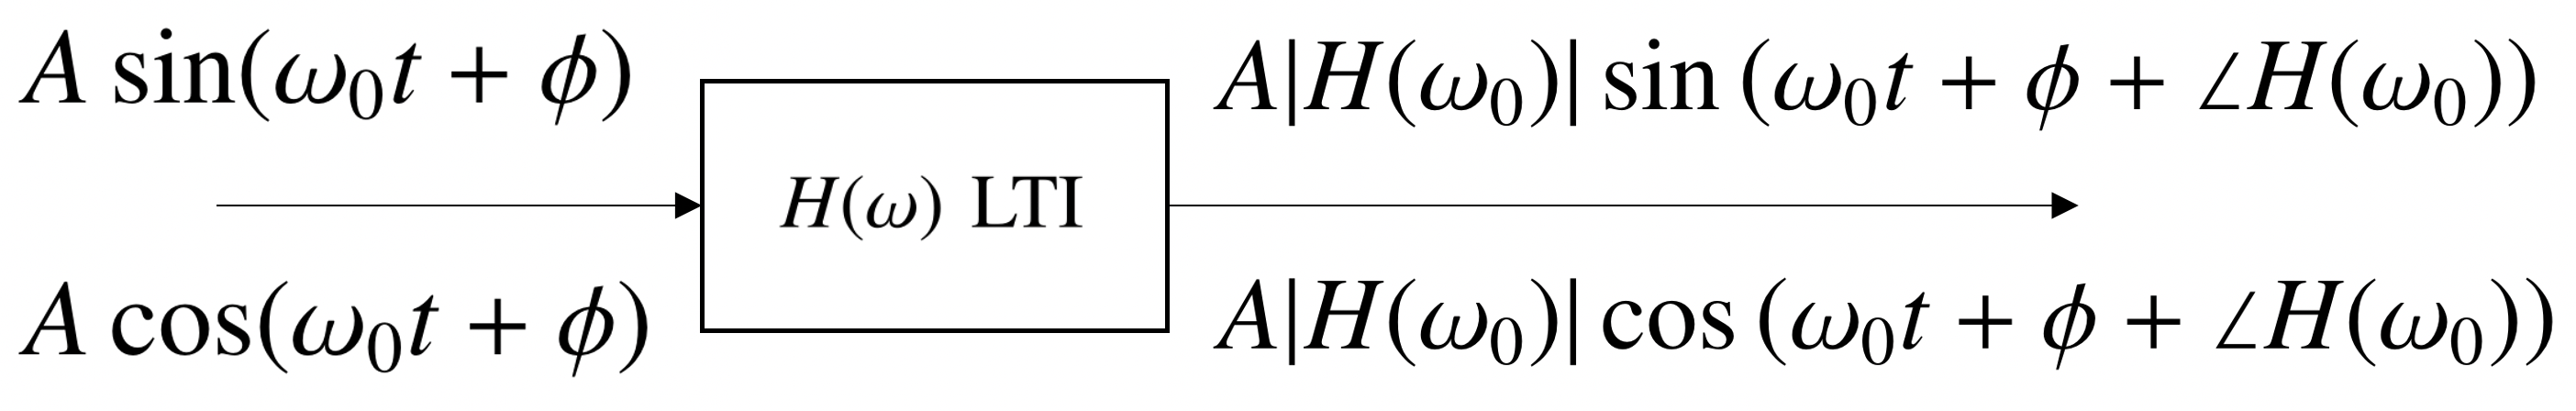
\includegraphics[width=\columnwidth]{figure.png}
         \caption{Output of LTI}
         \label{plot}
\end{figure}
\begin{enumerate}
    \item 
        For input signal $8\cos\left(20\pi t+\dfrac{\pi}{4}\right)$,
        \begin{align}
            f_1=20\pi/2\pi=10\text{Hz}
        \end{align}
        Since $|f_1|\leq20$,
        \begin{align}
            |H(f_1)|=1-\dfrac{10}{20}=\dfrac{1}{2}
        \end{align}
        Also,
        \begin{align}
            \arg H(f_1)=-2f_1=-20
        \end{align}
        So, the output signal $y_1(t)$ is 
        \begin{align}
            y_1(t)&=\left(8\times\dfrac{1}{2}\right)\cos\left(20\pi t+\dfrac{\pi}{4}-20\right)\\
            \implies y_1(t)&= 4\cos\left(20\pi t+\dfrac{\pi}{4}-20\right)
        \end{align}
    \item
        For input signal $16\sin\left(40\pi t+\dfrac{\pi}{8}\right)$,
        \begin{align}
            f_2=40\pi/2\pi=20\text{Hz}
        \end{align}
        Since $|f_2|\leq20$,
        \begin{align}
            |H(f_2)|=1-\dfrac{20}{20}=0
        \end{align}
        So, the output signal $y_2(t)=0$.
    \item
        For input signal $24\cos\left(80\pi t+\dfrac{\pi}{16}\right)$,
        \begin{align}
            f_3=80\pi/2\pi=40\text{Hz}
        \end{align}
        Since $|f_3|>20$,
        \begin{align}
            |H(f_3)|=0
        \end{align}
        So, the output signal $y_3(t)=0$.
\end{enumerate}
So, the total output signal is
\begin{align}
    y(t)&=y_1(t)+y_2(t)+y_3(t)\\
    \implies y(t)&= 4\cos\left(20\pi t+\dfrac{\pi}{4}-20\right)
\end{align}
Average power of this output signal
\begin{align}
    P_{y(t)}=\dfrac{4^2}{2}=8\text{W}
\end{align}
\end{document}
